\documentclass[10pt]{book} 
\usepackage{times} 
\usepackage{geometry} 
\usepackage{titlesec} 
\usepackage{amsmath}
\usepackage{amsfonts}
\usepackage{graphicx,subcaption}
\usepackage{float}
\usepackage{tikz,lipsum,lmodern}
\usepackage[most]{tcolorbox}
\usepackage[colorlinks=true,linkcolor=blue, citecolor=blue]{hyperref}
\usepackage[authoryear,round]{natbib}

\usepackage{titlesec}

% Adjust spacing for chapters
\titlespacing*{\chapter}{0pt}{-50pt}{20pt}

% Adjust spacing for sections
\titlespacing*{\section}{0pt}{20pt}{10pt}


% Remove paragraph indentation and add space between paragraphs
\setlength{\parindent}{0pt}
\setlength{\parskip}{\baselineskip}

\geometry{left=1.25in, right=1in, top=1in, bottom=1in}

\titleformat{\chapter}[display]
{\normalfont\Large\bfseries}{\chaptertitlename\ \thechapter}{20pt}{\Large}
\titleformat{\section}
{\normalfont\large\bfseries}{\thesection}{1em}{}

\title{A Comprehensive Note on Machine Learning\footnote{This content serve only for educational and personal purpose, \textbf{do not share} without my approval.}}
\author{Jue Guo}
\date{\today}

\begin{document}
\frontmatter
\maketitle
\tableofcontents
\chapter*{Preface}

The primary purpose of this document is educational, specifically for the courses I teach (\textbf{CSE 474/574 Introduction to Machine Learning, CSE 455/555 Pattern Recognition, and CSE 676 Deep Learning}), as well as for my personal reference. A substantial portion of the material herein is directly referenced or adapted from established texts and sources, and is not claimed as original content. This document is intended as a supplementary teaching and learning resource and is not authorized for commercial use, redistribution, or sale without my explicit consent.

The majority of the material referenced comes from the following sources:

{
\renewcommand{\labelenumi}{[\theenumi]}
\setcounter{enumi}{0} % Start enumeration from 1

\begin{enumerate}
	\item Zhang, Aston, et al. Dive into deep learning. Cambridge University Press, 2023.
	\item Bishop, C. M., \& Nasrabadi, N. M. (2006). Pattern recognition and machine learning (Vol. 4, No. 4, p. 738). New York: Springer.
	\item Hart, P. E., Stork, D. G., \& Duda, R. O. (2000). Pattern classification. Hoboken: Wiley.
	\item Burkov, A. (2019). The hundred-page machine learning book (Vol. 1, p. 32). Quebec City, QC, Canada: Andriy Burkov.
	\item Burkov, A. (2020). Machine learning engineering (Vol. 1). Montreal, QC, Canada: True Positive Incorporated.
\end{enumerate}
}

All other referenced materials and sources are cited in the bibliography section of this document. This compilation is intended to provide a comprehensive overview and guide for students and practitioners of machine learning, drawing upon a wide range of foundational and contemporary sources in the field.

\mainmatter
\part{Basic Machine Learning}
\chapter{Introduction}
\section{What is Machine Learning}
Machine learning is a subfield of computer science that is concerned with building algorithms which to be useful, rely on a collection of examples of some phenomenon.
\begin{itemize}
	\item The examples come from nature, handcrafted by humans or generated by another algorithms.
\end{itemize}
Machine learning can also be defined as the process of solving a practical problem by
\begin{enumerate}
	\item gathering a dataset
	\item algorithmically building a statistical model based on the dataset.
\end{enumerate}
The statistical model is assumed to be used somehow to solve the practical problem.
\section{Types of Learninig}
Learning can be \textbf{supervised}, \textbf{semi-supervised}, \textbf{unsupervised} and \textbf{reinforcement}.
\subsection{Supervised Learning}
In \textbf{supervised learning}, the \textbf{dataset} is the collection of \textbf{labeled examples} $\left\{\left(\mathbf{x}_i, y_i\right)\right\}_{i=1}^N$.
\begin{itemize}
	\item Each element $\mathbf{x}_i$ among $N$ is called a \textbf{feature vector}. A feature vector is a vector in which each dimension $j=1,...,D$ contains a value that describes the example somehow. That value is called a \textbf{feature} and is denoted as \(x^{(j)}\).
	\item The \textbf{label} \(y_i\) can be either an element belonging to a finite set of \textbf{classes} ${1,2,...,C}$, or a real number, or a more complex structure, like a vector, a matrix, a tree or a graph. Unless otherwise stated, $y_i$ is either one of a finite set of classes or a real number.
\end{itemize}
The goal of a \textbf{supervised learning algorithm} is to use the dataset to produce a \textbf{model} that takes a feature vector $\mathbf{x}$ as input and outputs information that allows deducing the label for this feature vector.

\subsection{Unsupervised Learning}
In \textbf{unsupervised learning}, the dataset is a collection of \textbf{unlabeled examples} $\left\{\mathbf{x}_i\right\}_{i=1}^N$. The goal of an \textbf{unsupervised learning algorithm} is to create a model that takes a feature vector $\mathbf{x}$ as input and either transforms it into another vector or into a value that can be used to solve a practical problem. For example,
\begin{itemize}
	\item in \textbf{clustering}, the model returns the id of the cluster for each feature vector in the dataset.
	\item in \textbf{dimensionality reduction}, the output of the model is a feature vector that has fewer features than the input $\mathbf{x}$;
	\item in \textbf{outlier detection}, the output is a real number that indicates how $\mathbf{x}$ is different from a ``typical" example in the dataset.
\end{itemize}
\subsection{Semi-Supervised Learning}
In \textbf{semi-supervised learning}, the dataset contains both labeled and unlabeled examples.
\begin{itemize}
	\item Usually the quantity of unlabeled examples is much higher than the number of labeled examples.
\end{itemize}
The goal of \textbf{semi-supervised learning algorithm} is the same as the goal of the supervised learning algorithm.
\begin{itemize}
	\item The hope here is that using many unlabeled examples can help the learning algorithm to find a better model.
\end{itemize}
How does the learning benefit from adding more unlabeled examples?
\begin{itemize}
	\item By adding unlabeled examples, you add more information about your problem:\textit{ a larger sample reflects better the probability distribution the data we labeled came from}.
\end{itemize}

\subsection{Reinforcement Learning}
\textbf{Reinforcement learning} is a subfield of machine learning where the machine ``lives" in an environment and is capable of perceiving the \textit{state} of that environment as vector of features.
\begin{itemize}
	\item The machine can execute \textit{actions} in every state. Different actions bring different \textit{rewards} and could also move the machine to another state of the environment.
\end{itemize}
The goal of a reinforcement learning algorithm is to learn a \textit{policy}. A policy is a function (similar to the model in supervised learning) that takes the feature vector of a state as input and outputs an optimal action to execute in that state. The action is optimal if it maximizes the \textit{expected average reward}.

\section{How Supervised Learning Works}
Supervised learning is the type of machine learning most frequently used in practice. The supervised learning process starts with gathering the data. The data for supervised learning is a collection of pairs (input,output).
\begin{itemize}
	\item Inputs could be anything, for example, email messages, pictures, or sensor measurements.
	\item Outputs are usually real numbers, or labels (e.g. ``spam", ``not\_spam", etc). In some cases, outputs are vectors (e.g., four coordinates of the rectangle around a person on the picture), sequences (e.g. [``adjective", ``adjective", ``noun"] for the input ``big beautiful car") or have some other structure.
\end{itemize}
You want to solve spam detection using supervised learning. First, you gather the data of 10,000 email messages and you have your label ``spam" or ``not\_spam" for each message. With the data at hand, you have to represent each message using a feature vector.

A common approach it to use \textbf{bag of words}, is to take a dictionary of English words (e.g. 20,000 alphabetically sorted words) and stipulate that in our feature vector:
\begin{itemize}
	\item the first feature is equal to 1 if the email message contains the word ``a"; other wise, this feature is 0;
	\item the second feature is equal to 1 if the email message contains the word ``aaron"; otherwise, this feature equals 0;
	\item ...
	\item the feature at position 20,000 is equal to 1 if the email message contains the word ``zulu"; otherwise, this feature is equal to 0.
\end{itemize}
You repeat the above procedure for every email message in our collection, which gives us 10,000 feature vectors (each vector having the dimensionality of 20,000) and a label (``spam"/``not\_spam").

We successfully converted input data into machine-readable type, but the output labels are still in the form of human-readable text. Some learning algorithms require transforming labels into numbers. For demonstration purpose, we will use a supervised learning algorithm called \textbf{Support Vector Machine} (SVM). This algorithm requires the positive label (in our case it's ``spam") has the numeric value of +1 (one), and the negative label (``not\_spam") has the value of -1 (minus one).

You now have a \textbf{dataset} and a \textbf{learning algorithm}, you will need to apply the learning algorithm to the dataset to get the \textbf{model}.

SVM sees every feature vector as a point in a high-dimensional space (in our case, space is 20,000 -- dimensional). The algorithm puts all feature vectors on an imaginary 20,000-dimensional plot and draws an imaginary 19,999 -- dimensional line (a \textit{hyperplane}) that separates examples with positive labels from examples with negative labels. In machine learning, the boundary separating the examples of different classes is called the \textbf{decision boundary}.

Hyperplane is denoted by two \textbf{parameters}

\[ \mathbf{w} \mathbf{x}-b=0 \text {, } \]
\begin{itemize}
	\item a real-valued vector $\mathbf{w}$ of the same dimensionality as our input vector $\mathbf{x}$, and a real number $b$
	\item $\mathbf{w} \mathbf{x}= w^{(1)} x^{(1)}+w^{(2)} x^{(2)}+\ldots+w^{(D)} x^{(D)}$, and $D$ is the number of dimensions of the feature vector $\mathbf{x}$.
\end{itemize}
The predicted label for some input feature vector $\mathbf{x}$ is given like this:

$$
	y=\operatorname{sign}(\mathbf{w} \mathbf{x}-b),
$$

where \verb*|sign| is a mathematical operator that takes any value as input and returns $+1$ if the input is a positive number or $-1$ if the input is a negative number.

The goal of the learning algorithm, SVM in this case, is to leverage the dataset and find the optimal values \(\mathbf{w}^{*}\) and $b^{*}$ for parameters $\mathbf{w}$ and $b$. Once the learning algorithm identifies these optimal values, the \textbf{model} $f(\mathbf{x})$ is then defined as:

\begin{equation*}
	f(\mathbf{x})=\operatorname{sign}\left(\mathbf{w}^* \mathbf{x}-b^*\right)
\end{equation*}


How do we find these optima values? It turns out it is an optimization problem. Machines are good at optimizing functions \underline{under constraints}.

$$
	\begin{array}{ll}
		\mathbf{w} \mathbf{x}_{i}-b \geq+1 & \text { if } y_{i}=+1 \\
		\mathbf{w} \mathbf{x}_{i}-b \leq-1 & \text { if } y_{i}=-1
	\end{array}
$$

It will also be ideal if the hyperplane separates positive examples from negative ones with the largest \textbf{margin}. The margin is the distance between the closestt examples of two classes, as defined by the decision boundary. A large margin contributes to a better \textbf{generalization}, that is how well the model will classify new examples in the future.

\begin{figure}[H]
	\centering
	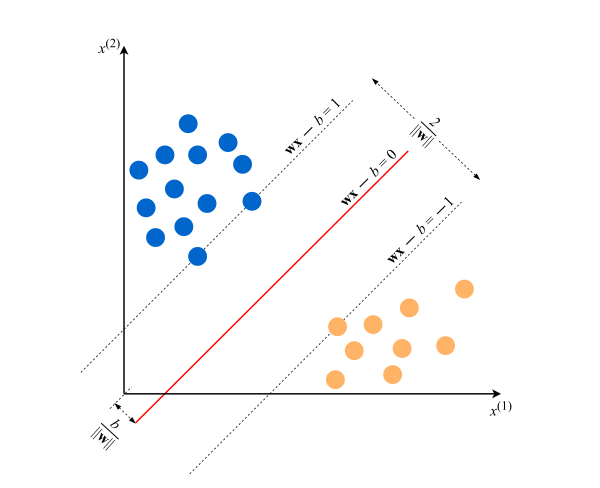
\includegraphics[width=0.7\linewidth]{imgs/introduction/intro_1}
	\caption{An example of an SVM model for two-dimensional feature vectors.}
	\label{fig:intro1}
\end{figure}

Let's do some quick refreshment
\vspace*{1em}
\begin{tcolorbox}[enhanced jigsaw, breakable, pad at break*=1mm, colback=gray!20!white, colframe=black!85!black, title=\textbf{Distance Formulas in Euclidean Space}]
	\textbf{Distance Between Two Points} \\
	In two-dimensional space, for points \( P_1(x_1, y_1) \) and \( P_2(x_2, y_2) \), the distance is calculated as:
	\[ d = \sqrt{(x_2 - x_1)^2 + (y_2 - y_1)^2} \]

	\textbf{Distance From a Point to a Line} \\
	In two-dimensional space, for a line defined by \( ax + by + c = 0 \) and a point \( P(x_0, y_0) \), the distance is:
	\[ d = \frac{|ax_0 + by_0 + c|}{\sqrt{a^2 + b^2}} \]

	\textbf{Distance Between Two Parallel Lines} \\
	For two parallel lines with equations \( ax + by + c_1 = 0 \) and \( ax + by + c_2 = 0 \), the distance is:
	\[ D = \frac{|c_2 - c_1|}{\sqrt{a^2 + b^2}} \]
\end{tcolorbox}
\vspace*{1em}
So, the optimization problem that we want the machine to solve looks like this:

\textit{\textbf{Minimize} $\|\mathbf{w}\|$ subject to $y_{i}\left(\mathbf{w} \mathbf{x}_{i}-b\right) \geq 1$ for $i=1, \ldots, N$. The expression $y_{i}\left(\mathbf{w} \mathbf{x}_{i}-b\right) \geq 1$ is just a compact way to write the above two constraints.}

More on SVMs later. This simple example should give you an idea how supervised learning works.

\section{Why the Model Works on New Data}

Let's refer to Figure \ref{fig:intro1}. If two classes are separable from one another by a decision boundary, then, obviously, examples that belong to each class are located in two different subspaces which the decision boundary creates.

If the examples used for training were selected randomly, independently of one another, and following the same procedure, then statistically, it is \textit{more likely} that the new negative example will be located on the plot somewhere not too far from other negative examples.  The idea goes with the positive examples as well.


\chapter{Notation and Definition}

\section{Notation}

We will review all the necessary notation and mathematics for us to continue the journey of Machine Learning.

\subsection{Data Structure}

A \textbf{scalar} is simple numerical value, like $15$ or $-3.25$, denoted by an italic letter, like $x$ or $a$. A \textbf{vector} is an ordered list of scalar values, called attributes. Vector is denoted by bold character $\mathbf{x}$ or $\mathbf{w}$. A \textbf{matrix} is a rectangular array of numbers arranged in rows and columns.

\begin{figure}[H]
	\begin{subfigure}[t]{0.45\linewidth}
		\centering
		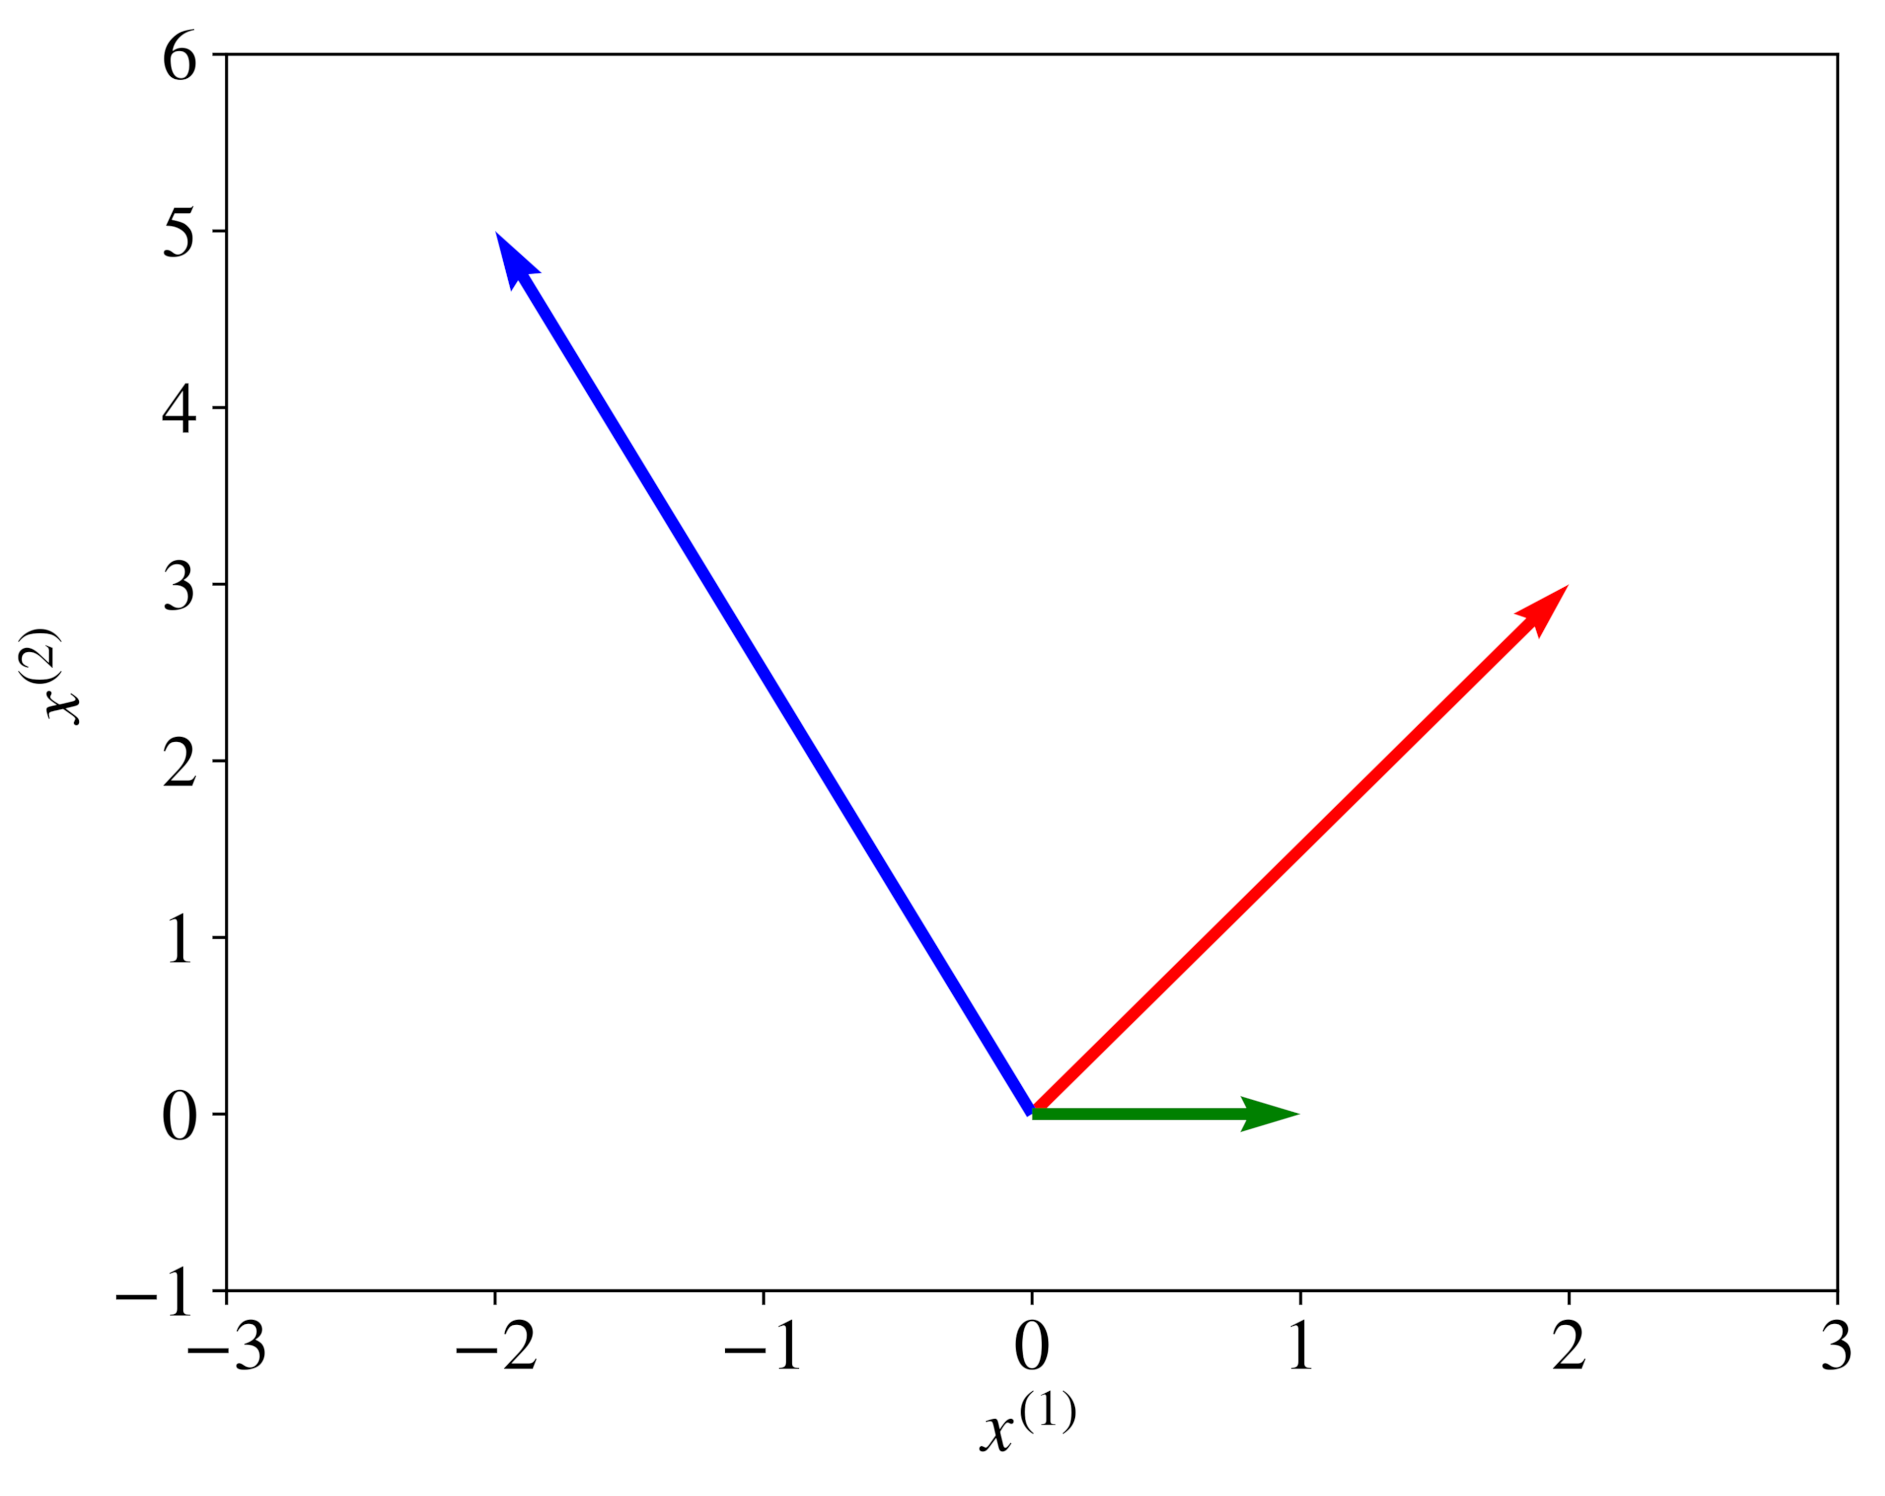
\includegraphics[width=\linewidth]{imgs/notation/notation_1}
		\caption{First subfigure}
	\end{subfigure}
	\hfill % this will put some space between your two figures
	\begin{subfigure}[t]{0.45\linewidth}
		\centering
		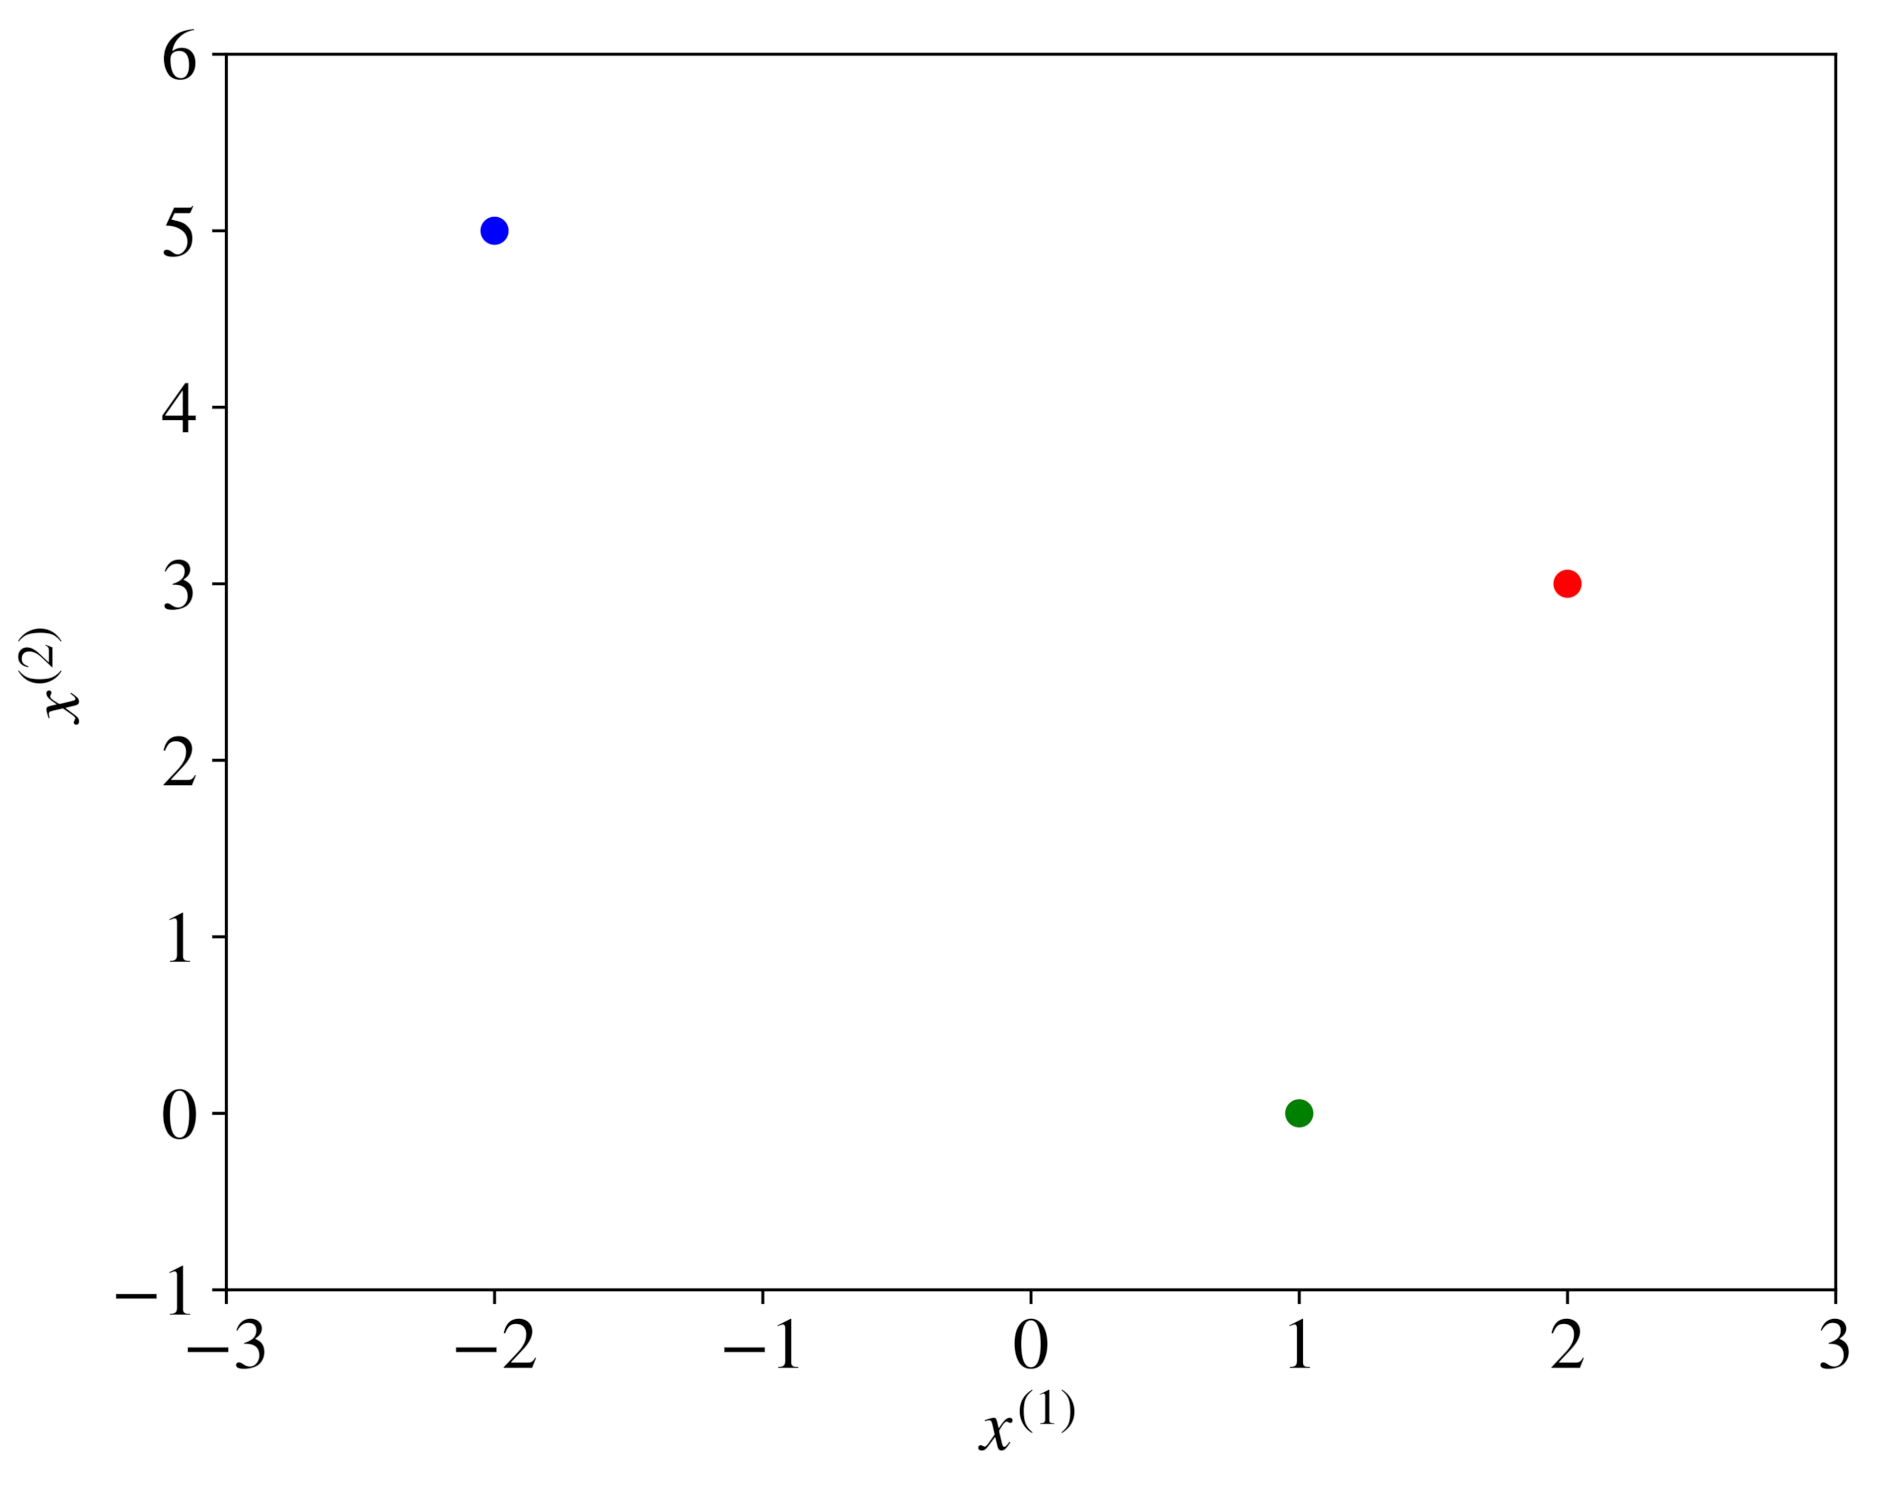
\includegraphics[width=\linewidth]{imgs/notation/notation_2}
		\caption{Second subfigure}
	\end{subfigure}
	\caption{Three vectors visualized as directions and as points.}
	\label{fig:notation_1}
\end{figure}

A \textbf{matrix} is a rectangular array of numbers arranged in rows and columns, which are denoted with bold capital letters, such as $\mathbf{A}$ or $\mathbf{W}$.  A \textbf{set} is an unordered collection of unique elements. We denote a set as a calligraphic capital character, for example, \(\mathcal{S}\). When an element belongs to a set \(\mathcal{S}\) , we write $x\in\mathcal{S}$. We can obtain a new set $\mathcal{S}_3$ as an \textbf{intersection} of two set $\mathcal{S}_1$ and $\mathcal{S}_2$, written as $\mathcal{S} \leftarrow\mathcal{S}_{1} \cap \mathcal{S}_{2}$. Also we can obtain a new set by \textbf{union}, $\mathcal{S}_3\leftarrow\mathcal{S}_1\cup\mathcal{S}_2$.

\subsection{Capital Sigma Notation}
The summation over a collection \(\mathcal{X}=\left\{x_{1}, x_{2}, \ldots, x_{n-1}, x_{n}\right\}\) or over the attributes of a vector $\mathbf{x}=\left[x^{(1)}, x^{(2)}, \ldots, x^{(m-1)}, x^{(m)}\right]$ is denoted like this:
\begin{equation*}
	\sum_{i=1}^{n} x_{i} \stackrel{\text { def }}{=} x_{1}+x_{2}+\ldots+x_{n-1}+x_{n}, \text { or else: } \sum_{j=1}^{m} x^{(j)} \stackrel{\text { def }}{=} x^{(1)}+x^{(2)}+\ldots+x^{(m-1)}+x^{(m)}
\end{equation*}
The notation $\stackrel{\text { def }}{=}$ means ``is defined as".

\subsection{Capital Pi Notation}

\begin{equation*}
	\prod_{i=1}^{n} x_{i} \stackrel{\text { def }}{=} x_{1} \cdot x_{2} \cdot \ldots \cdot x_{n-1} \cdot x_{n}
\end{equation*}
\begin{itemize}
	\item A product of elements in a collection or attributes of a vector.
\end{itemize}

\subsection{Operations on Sets}

Given the expression:
\[ \mathcal{S}^{\prime} \leftarrow \left\{x^{2} \mid x \in \mathcal{S}, x > 3\right\} \]
This notation is used to define a derived set creation operator. It means that we create a new set \( \mathcal{S}^{\prime} \) by including the square of each element \( x \) from the set \( \mathcal{S} \), under the condition that \( x \) is greater than 3. In other words, \( \mathcal{S}^{\prime} \) is comprised of the squares of all elements in \( \mathcal{S} \) which are greater than 3.

Additionally, the cardinality operator \( |\mathcal{S}| \) is used to denote the number of elements in the set \( \mathcal{S} \). For example, if \( \mathcal{S} = \{1, 2, 4, 5\} \), then \( \mathcal{S}^{\prime} = \{16, 25\} \) as only 4 and 5 from \( \mathcal{S} \) satisfy the condition \( x > 3 \). The \textbf{cardinality} \( |\mathcal{S}| \) in this case would be 4.

\subsection{Operations on Vectors}

\textbf{Vector Addition and Subtraction:}
The sum and difference of two vectors \( \mathbf{x} \) and \( \mathbf{z} \) are defined component-wise as:
\[ \mathbf{x} + \mathbf{z} = \left[x^{(1)} + z^{(1)}, \ldots, x^{(m)} + z^{(m)}\right] \]
\[ \mathbf{x} - \mathbf{z} = \left[x^{(1)} - z^{(1)}, \ldots, x^{(m)} - z^{(m)}\right] \]
\emph{Example:} For \( \mathbf{x} = [1, 2] \) and \( \mathbf{z} = [3, 4] \),
\[ \mathbf{x} + \mathbf{z} = [1+3, 2+4] = [4, 6] \]

\textbf{Scalar Multiplication:}
A vector multiplied by a scalar \( c \) results in a scaled vector:
\[ \mathbf{x} c = \left[c x^{(1)}, \ldots, c x^{(m)}\right] \]
\emph{Example:} For \( \mathbf{x} = [1, 2] \) and \( c = 3 \),
\[ \mathbf{x} c = [3 \times 1, 3 \times 2] = [3, 6] \]

\textbf{Dot Product:}
The dot product of two vectors \( \mathbf{w} \) and \( \mathbf{x} \) is a scalar:
\[ \mathbf{w} \mathbf{x} = \sum_{i=1}^{m} w^{(i)} x^{(i)} \]
\emph{Example:} For \( \mathbf{w} = [1, 2] \) and \( \mathbf{x} = [3, 4] \),
\[ \mathbf{w} \mathbf{x} = 1 \times 3 + 2 \times 4 = 3 + 8 = 11 \]
\textbf{Matrix-Vector Multiplication:}
Multiplying a matrix \( \mathbf{W} \) by a vector \( \mathbf{x} \) yields another vector. For example:
$$
	\begin{aligned}
		\mathbf{W} \mathbf{x} & =\left[\begin{array}{lll}
				                               w^{(1,1)} & w^{(1,2)} & w^{(1,3)} \\
				                               w^{(2,1)} & w^{(2,2)} & w^{(2,3)}
			                               \end{array}\right]\left[\begin{array}{l}
				                                                       x^{(1)} \\
				                                                       x^{(2)} \\
				                                                       x^{(3)}
			                                                       \end{array}\right]                                      \\
		                      & \stackrel{\text { def }}{=}\left[\begin{array}{l}
				                                                         w^{(1,1)} x^{(1)}+w^{(1,2)} x^{(2)}+w^{(1,3)} x^{(3)} \\
				                                                         w^{(2,1)} x^{(1)}+w^{(2,2)} x^{(2)}+w^{(2,3)} x^{(3)}
			                                                         \end{array}\right] \\
		                      & =\left[\begin{array}{l}
				                               \mathbf{w}^{(1)} \mathbf{x} \\
				                               \mathbf{w}^{(2)} \mathbf{x}
			                               \end{array}\right]
	\end{aligned}
$$

\emph{Example:} For
\[ \mathbf{W} = \left[\begin{array}{ll}
			1 & 2 \\
			3 & 4
		\end{array}\right] \text{ and } \mathbf{x} = \left[\begin{array}{l}
			5 \\
			6
		\end{array}\right], \]
\[ \mathbf{W} \mathbf{x} = \left[\begin{array}{l}
			1 \times 5 + 2 \times 6 \\
			3 \times 5 + 4 \times 6
		\end{array}\right] = \left[\begin{array}{l}
			17 \\
			39
		\end{array}\right] \]
\textbf{Transpose and Multiplication:}
For the transpose of a vector \( \mathbf{x} \) denoted \( \mathbf{x}^{\top} \), and a matrix \( \mathbf{W} \), the multiplication \( \mathbf{x}^{\top} \mathbf{W} \) is given by:
$$
	\begin{aligned}
		\mathbf{x}^{\top} \mathbf{W} & =\left[\begin{array}{ll}
				                                      x^{(1)} & x^{(2)}
			                                      \end{array}\right]\left[\begin{array}{lll}
				                                                              w^{(1,1)} & w^{(1,2)} & w^{(1,3)} \\
				                                                              w^{(2,1)} & w^{(2,2)} & w^{(2,3)}
			                                                              \end{array}\right]                                                                                      \\
		                             & \stackrel{\text { def }}{=}\left[w^{(1,1)} x^{(1)}+w^{(2,1)} x^{(2)}, w^{(1,2)} x^{(1)}+w^{(2,2)} x^{(2)}, w^{(1,3)} x^{(1)}+w^{(2,3)} x^{(2)}\right]
	\end{aligned}
$$

\emph{Example:} For
\[ \mathbf{x} = \left[\begin{array}{l}
			7 \\
			8
		\end{array}\right] \text{ and } \mathbf{W} = \left[\begin{array}{lll}
			1 & 2 & 3 \\
			4 & 5 & 6
		\end{array}\right], \]
\[ \mathbf{x}^{\top} \mathbf{W} = \left[\begin{array}{lll}
			7 \times 1 + 8 \times 4, 7 \times 2 + 8 \times 5, 7 \times 3 + 8 \times 6
		\end{array}\right] = \left[\begin{array}{lll}
			39, 54, 69
		\end{array}\right] \]

\subsection{Functions}

\textbf{Definition of a Function}\\
A function is a relation that associates each element \( x \) of a set \( \mathcal{X} \), known as the domain, to a single element \( y \) of another set \( \mathcal{Y} \), known as the codomain. This relation is denoted as \( y = f(x) \), where \( f \) is the name of the function, \( x \) is the input or argument, and \( y \) is the output. The input variable is also referred to as the variable of the function.

\emph{Example:} Consider the function \( f(x) = x^2 \) defined on the domain \( \mathcal{X} = \mathbb{R} \). For \( x = 2 \), the output is \( f(2) = 2^2 = 4 \).

\textbf{Local and Global Minima}\\
The function \( f(x) \) has a local minimum at \( x = c \) if \( f(x) \geq f(c) \) for every \( x \) in an open interval around \( c \). An open interval, such as \( (0,1) \), includes all numbers between its endpoints but not the endpoints themselves. The smallest value among all local minima is known as the global minimum.

\emph{Example:} In the function \( f(x) = (x-1)^2 \), the local (and global) minimum occurs at \( x = 1 \) since \( f(x) \geq f(1) = 0 \) for all \( x \).

\begin{figure}[H]
	\centering
	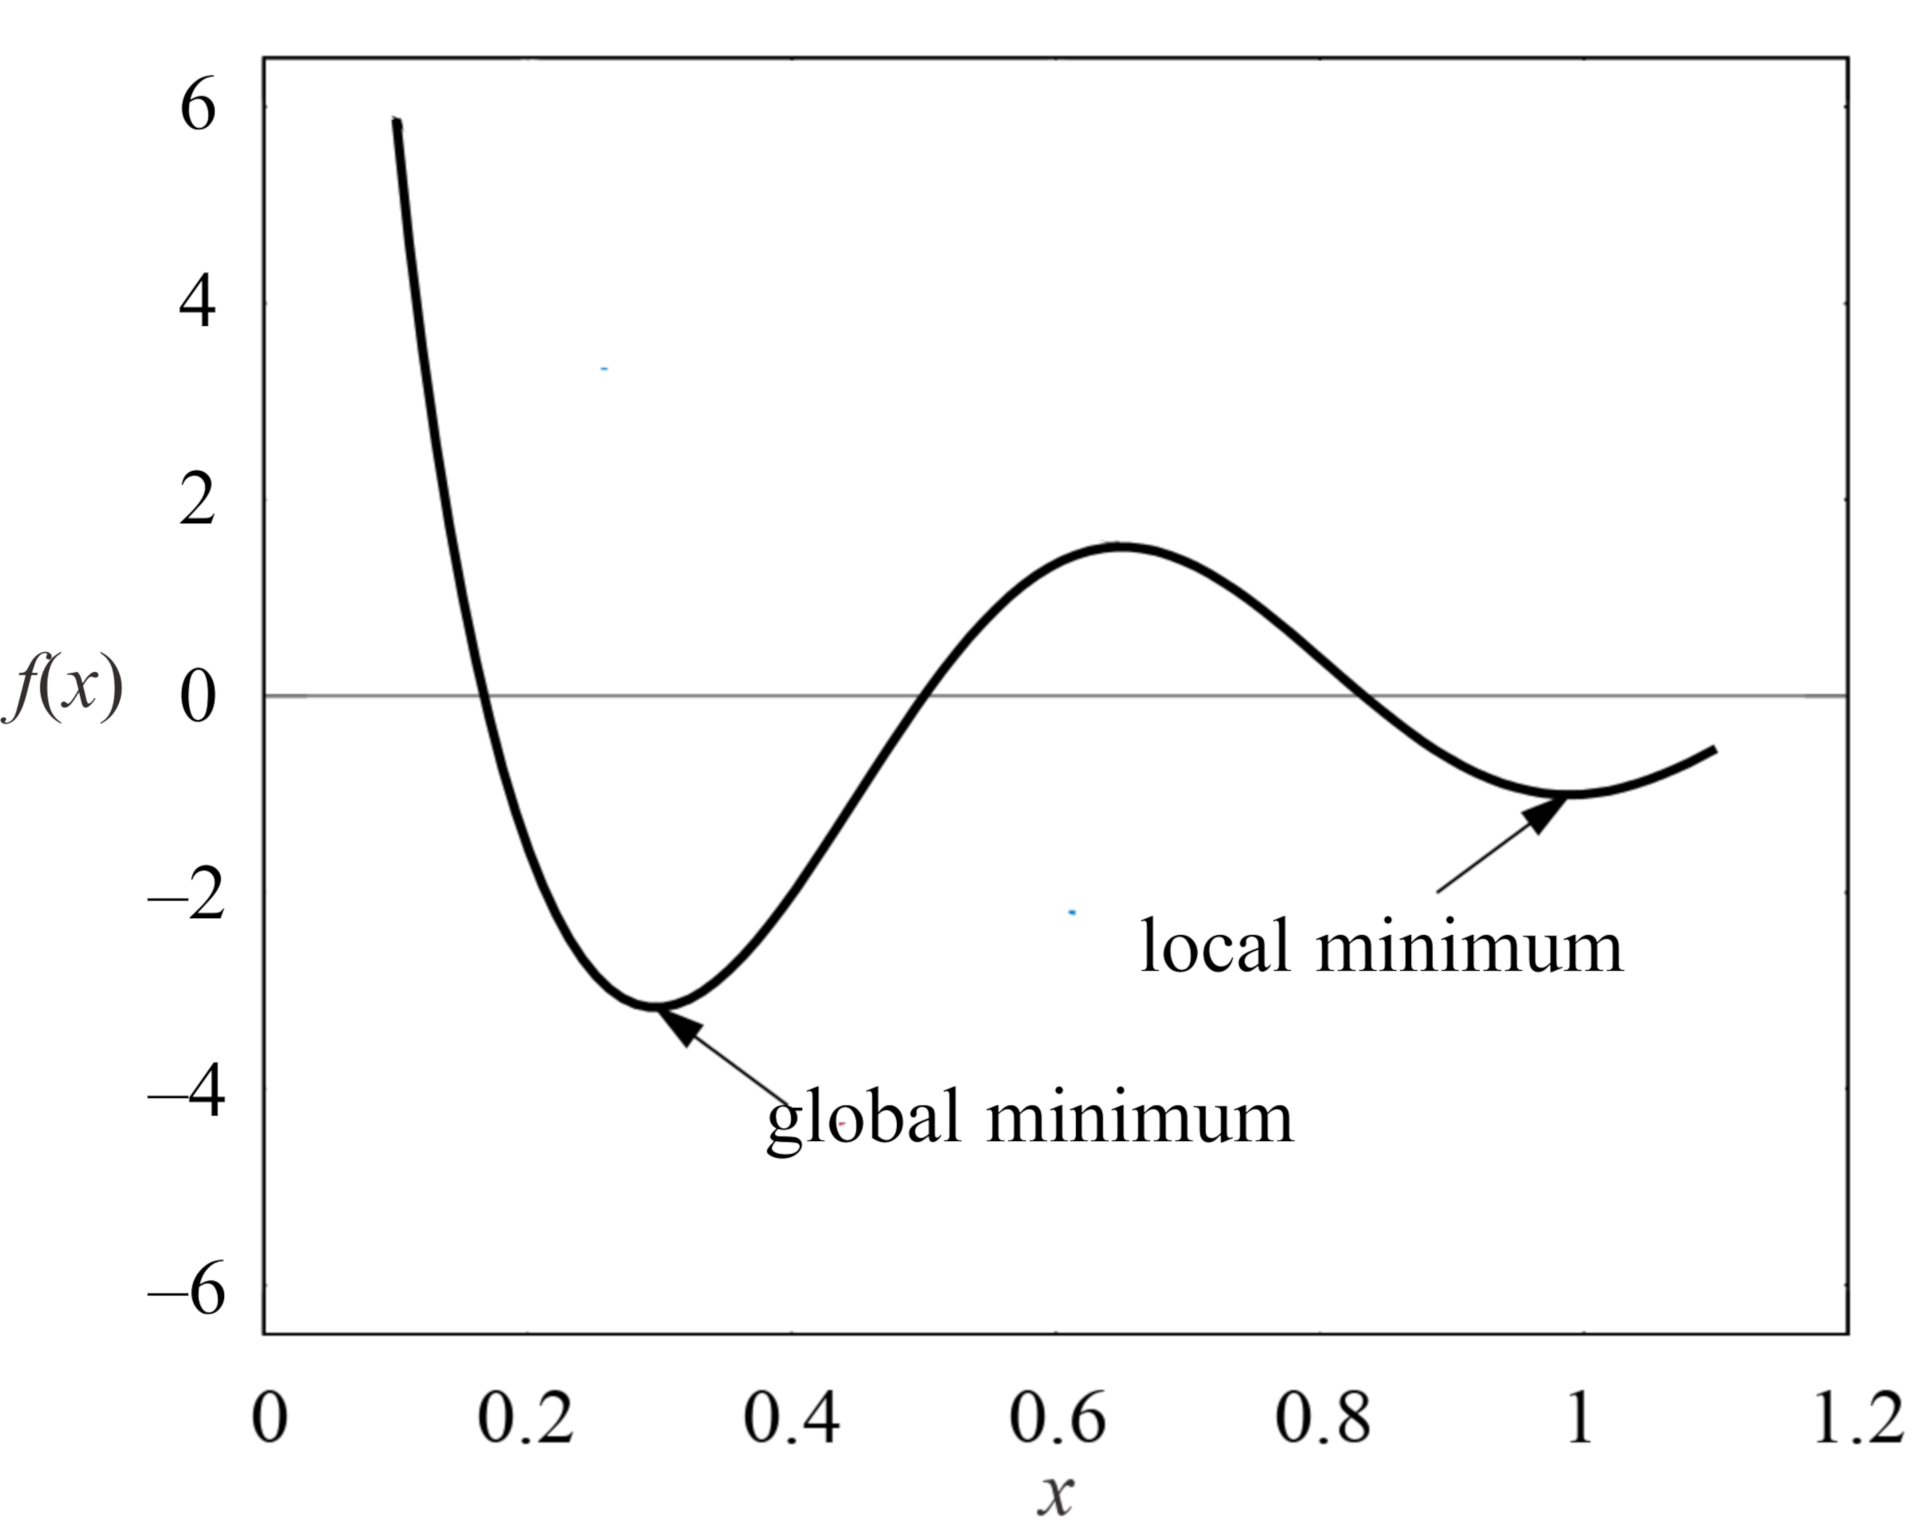
\includegraphics[width=0.7\linewidth]{imgs/notation/notation_3.png}
	\caption{A local and a global minima of a function.}
	\label{fig:notation_3}
\end{figure}

\textbf{Vector Functions}\\
A vector function, denoted \( \mathbf{y} = \mathbf{f}(x) \), is a function that returns a vector \( \mathbf{y} \). Its argument can be either a vector or a scalar.

\emph{Example:} For the vector function \( \mathbf{f}(x) = [x, x^2] \), with \( x = 2 \), the output is \( \mathbf{f}(2) = [2, 2^2] = [2, 4] \).

\subsection{Max and Arg Max}

Given a set of values \( \mathcal{A} = \{a_{1}, a_{2}, \ldots, a_{n}\} \), the operator \( \max_{a \in \mathcal{A}} f(a) \) returns the highest value of \( f(a) \) for all elements in the set \( \mathcal{A} \). Conversely, the operator \( \arg \max_{a \in \mathcal{A}} f(a) \) identifies the specific element \( a \) in the set \( \mathcal{A} \) that maximizes the function \( f(a) \).

In cases where the set is implicit or infinite, we can use the notation \( \max_{a} f(a) \) or \( \arg \max_{a} f(a) \) respectively. Similarly, the operators \( \min \) and \( \arg \min \) function in a comparable way, determining the lowest value of a function and the

\subsection{Assignment Operator}
The expression \(a \leftarrow f(x)\) means that the variable \(a\) gets the new value: the result of \(f(x)\). We say that the variable \(a\) gets assigned a new value. Similarly, \(\mathbf{a} \leftarrow\left[a_{1}, a_{2}\right]\) means that the vector variable \(\mathbf{a}\) gets the two-dimensional vector \(\left[a_{1}, a_{2}\right]\).

\subsection{Derivative and Gradient}
A \textbf{derivative} \(f^{\prime}\) of a function \(f\) is a function or a value that describes how fast \(f\) grows (or decreases).
\part{Advance Machine Learning}
\part{Convolution Neural Networks}
\part{Adversarial Attacks and Training}
\chapter{Intriguing Properties of Neural Network}

Deep neural networks, known for their exceptional performance in speech and visual recognition tasks, exhibit two notable characteristics \citep{szegedy2013intriguing}. First, \textit{the semantic information in their higher layers is embedded not in individual units but in the collective space they form}. This insights shifts the focus from analyzing single neurons to considering the entire unit group to understand network processing. Second, \textit{these networks display a surprisingly sensitivity to minute, yet percisely tailored alternations (or perturbation).} Such small changes can lead to incorrect outcomes. This vulnerability is not due to random noise; the same modifications can deceive different networks trained on a different subset of the dataset, to misclassify the same input.

\section{Introduction}

Deep neural networks are powerful learning models that achieve excellent performance on visual and speech recognition problems because they can express arbitrary computation that consists of a modest number of massively parallel nonlinear steps. As the resulting computation is automatically discovered by backpropagation via supervised learning, it can be difficult to interpret and can have counter-intuitive properties.

The \textbf{first} property is concerned with the semantic meaning of individual units. It seems that the entire space of activation, rather than the individual units, that contains the bulk of the semantic information contrary to prior belief and the \textbf{second} property is concerned with the stability of neural networks with respect to small perturbation to their inputs. Apply an \textit{imperceptible} non-random perturbation to a test image, it is possible to arbitrarily change the network's prediction. These perturbation are found by optimizing the input to maximize the prediction error. The perturbed examples are often called ``adversarial examples"

\section{Framework}
\textbf{Notation} $x\in \mathbb{R}$ denotes an input image, $\phi(x)$ is an activation values of some layer. \citep{szegedy2013intriguing} first examine properties of the image of $\phi(x)$, and then search for its blind spots. 

\part{Recurrent Neural Networks}
\part{Transformers}
\part{Artificial General Intelligence}
\chapter{Continual Learning}
\section{Introduction}
\textbf{Continual Learning} is motivated by the fact that human and other organisms has the ability to adapt, accumulate and exploit knowledge. A common setting for continual learning is to learn a sequence of contents one by one and behave as if they were observed simultaneously \citep{wang2023comprehensive}. Each task learned throughout the life time can be new skills, new examples of old skills, different environments, etc (Fig.\ref{fig:cl_1}, a). This attribute of continual learning makes it also referred to as \textbf{incremental learning} or \textbf{lifelong learning}.

Unlike conventional pipeline, where joint training is applied, continual learning is characterized by learning from dynamic data distributions. A major challenge is known as \textbf{catastrophic forgetting}, where \textit{adaptation to a new distribution generally results in a largely reduced ability to capture the old ones}. This dilemma is a facet of the trade-off between \textbf{learning plasticity} and \textbf{memory stability}: an excess of the former interferes with the latter, and vice versa. A good continual learning algorithm should obtain a strong \textbf{generalizability} to accommodate distribution differences within and between tasks (Fig.\ref{fig:cl_1}, b). As a naive baseline, retraining all old training samples (if allowed) makes it easy to address the above challenges, but creates huge computational and storage overheads (as well as potential privacy issues). In fact, continual learning is primarily intended to ensure \textbf{resource efficiency} of model updates, preferably close to learning only new training samples.

\begin{figure}[H]
    \centering
    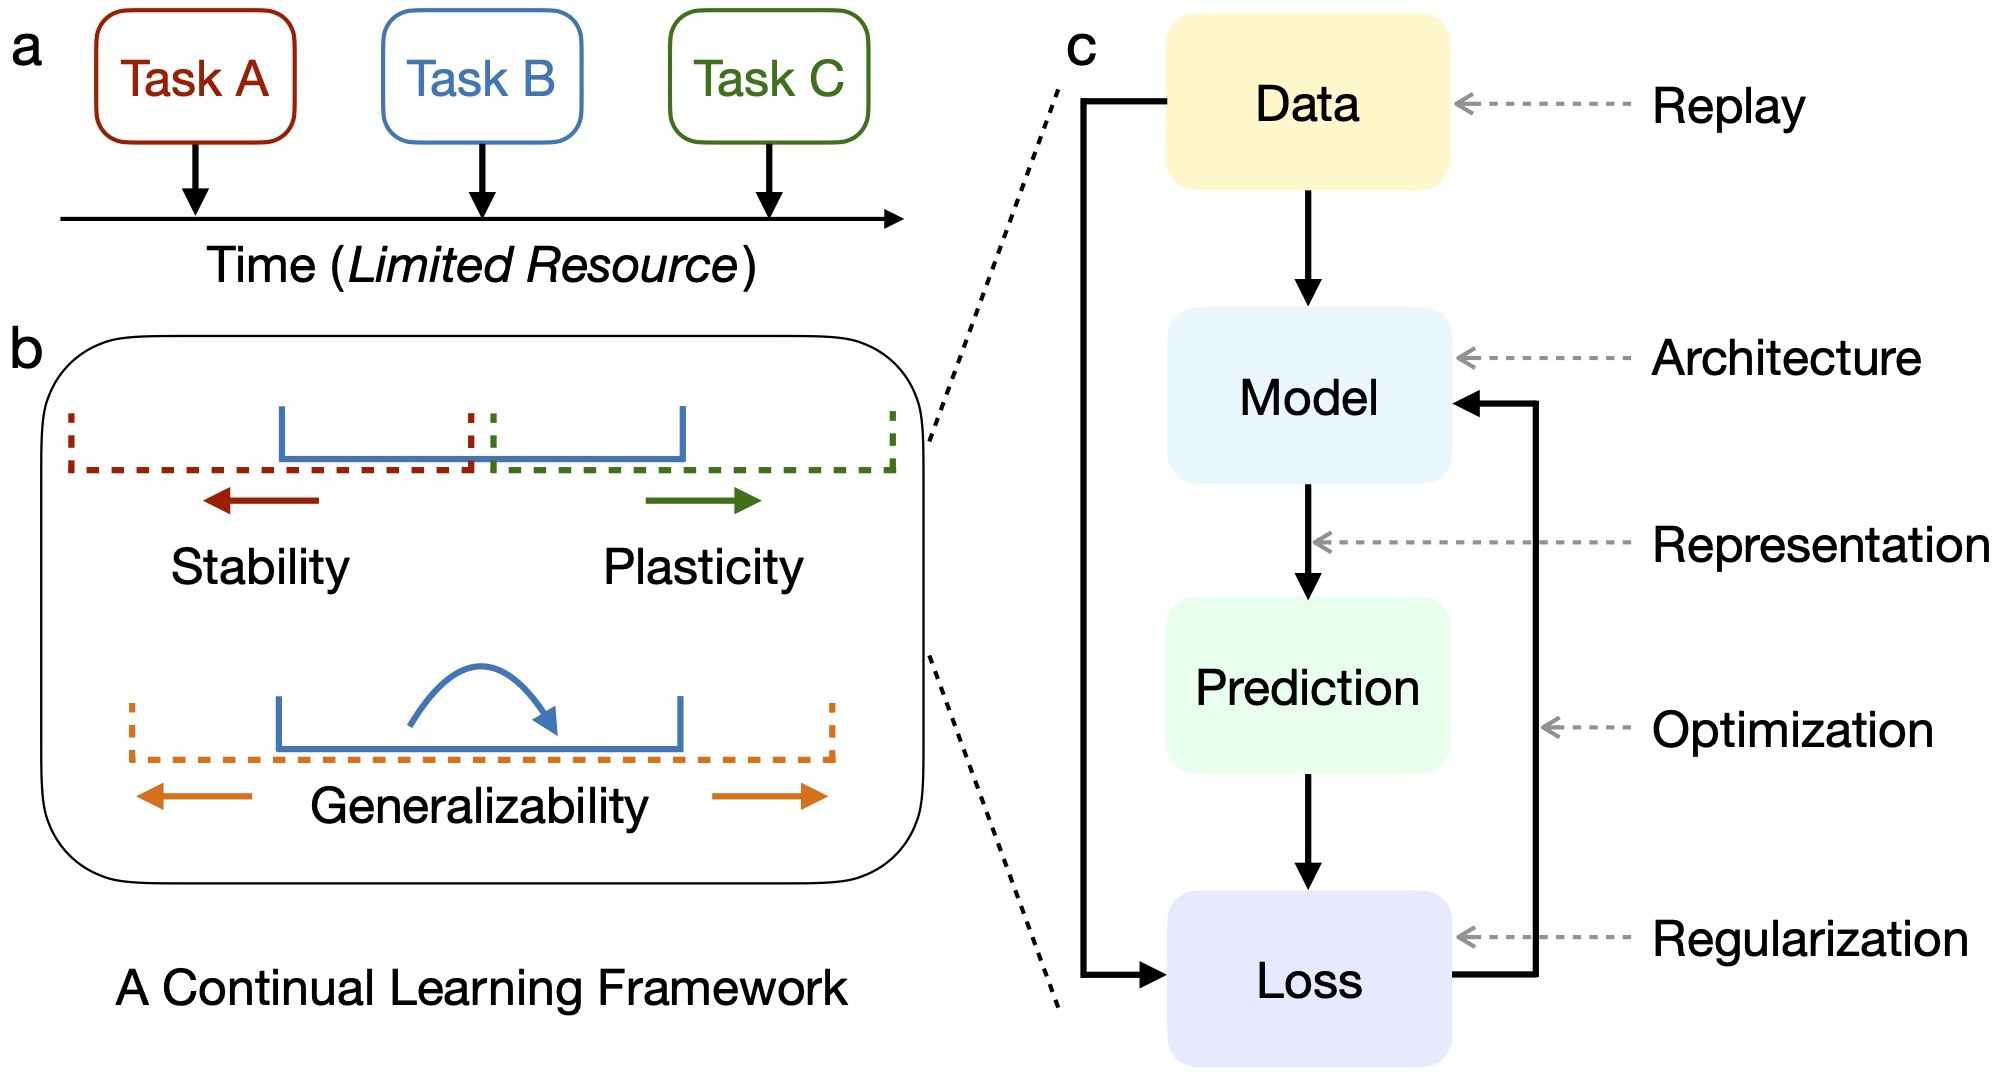
\includegraphics[width=0.7\linewidth]{imgs/continual_learning/cl_1.png}
    \caption{A conceptual framework of continual learning. \textbf{a}, Continual learning requires adapting to incremental tasks with dynamic data distributions. \textbf{b}, A desirable solution should ensure a proper balance between stability (red arrow) and plasticity (green arrow), as well as an adequate generalizability to intra-task (blue arrow) and inter-task (orange arrow) distribution differences. \textbf{c}, Representative strategies have targeted various aspects of machine learning.}
    \label{fig:cl_1}
\end{figure}

Numerous efforts have been devoted to addressing the above challenges, which can be conceptually separated into five groups (Fig.\ref{fig:cl_1}, c): \textit{regularization-based approach}; \textit{replay-based approach}; \textit{optimization-based approach}; \textit{representation-based approach}; and \textit{architecture-based approach}. These methods are \textit{closely connected}, e.g., regularization and replay ultimately act to rectify the gradient directions, and \textit{highly synergistic}, e.g., the efficacy of replay can be facilitated by distilling knowledge from the old model.

\section{Setup}
In this section, we first present a basic formulation of continual leanring. Then we introduce typical scenairos and evaluation metrics.

\subsection{Basic Formulation}
A continual learning model parameterized by \(\theta\) needs to learn corresponding task(s) with no or limited access to old training samples and perform well on their test sets. Formally, an incoming batch of training samples belonging to a task \(t\) can be represented as \(\mathcal{D}_{t, b}=\left\{\mathcal{X}_{t, b}, \mathcal{Y}_{t, b}\right\}\) where \(\mathcal{X}_{t, b}\) is the input data, \(\mathcal{Y}_{t, b}\) is the data label, \(t \in \mathcal{T}=\{1, \cdots, k\}\) is the task identity and \(b \in \mathcal{B}_{t}\) is the batch index ( \(\mathcal{T}\) and \(\mathcal{B}_{t}\) denote their space, respectively). Here we define a "task" by its training samples \(\mathcal{D}_{t}\) following the distribution \(\mathbb{D}_{t}:=p\left(\mathcal{X}_{t}, \mathcal{Y}_{t}\right)\left(\mathcal{D}_{t}\right.\) denotes the entire training set by omitting the batch index, likewise for \(\mathcal{X}_{t}\) and \(\left( \mathcal{Y}_{t}\right)\), and assume that there is no difference in distribution between training and testing. Under realistic constraints, the data label \(\mathcal{Y}_{t}\) and the task identity \(t\) might not be always available. In continual learning, the training samples of each task can arrive incrementally in batches (i.e., \(\left\{\left\{\mathcal{D}_{t, b}\right\}_{b \in \mathcal{B}_{t}}\right\}_{t \in \mathcal{T}}\) ) or simultaneously (i.e.,\(\left\{\mathcal{D}_{t}\right\}_{t \in \mathcal{T}}\)).

\begin{table}[H]
    \centering
    \renewcommand{\arraystretch}{1.75}
    \resizebox{\textwidth}{!}{
        \begin{tabular}{c|c|c}
            \hline
            \textbf{Scenario} & \textbf{Training}                                                                                                                                                                                                                               & \textbf{Testing}                                                                                  \\
            \hline IIL        & \(\left\{\left\{\mathcal{D}_{t, b}, t\right\}_{b \in \mathcal{B}_{t}}\right\}_{t=j}\)                                                                                                                                                           & \(\left\{p\left(\mathcal{X}_{t}\right)\right\}_{t=j ; t}\) is not required                        \\
            \hline DIL        & \(\left\{\mathcal{D}_{t}, t\right\}_{t \in \mathcal{T}} ; p\left(\mathcal{X}_{i}\right) \neq p\left(\mathcal{X}_{j}\right)\) and \(\mathcal{Y}_{i}=\mathcal{Y}_{j}\) for \(i \neq j\)                                                           & \(\left\{p\left(\mathcal{X}_{t}\right)\right\}_{t \in \mathcal{T}}, t\) is not required           \\
            \hline TIL        & \(\left\{\mathcal{D}_{t}, t\right\}_{t \in \mathcal{T}} ; p\left(\mathcal{X}_{i}\right) \neq p\left(\mathcal{X}_{j}\right)\) and \(\mathcal{Y}_{i} \cap \mathcal{Y}_{j}=\emptyset\) for \(i \neq j\)                                            & \(\left\{p\left(\mathcal{X}_{t}\right)\right\}_{t \in \mathcal{T} ; t}\) is available             \\
            \hline CIL        & \(\left\{\mathcal{D}_{t}, t\right\}_{t \in \mathcal{T}} ; p\left(\mathcal{X}_{i}\right) \neq p\left(\mathcal{X}_{j}\right)\) and \(\mathcal{Y}_{i} \cap \mathcal{Y}_{j}=\emptyset\) for \(i \neq j\)                                            & \(\left\{p\left(\mathcal{X}_{t}\right)\right\}_{t \in \mathcal{T} ; t}\) is unavailable           \\
            \hline TFCL       & \(\left\{\left\{\mathcal{D}_{t, b}\right\}_{b \in \mathcal{B}_{t}}\right\}_{t \in \mathcal{T}} ; p\left(\mathcal{X}_{i}\right) \neq p\left(\mathcal{X}_{j}\right)\) and \(\mathcal{Y}_{i} \cap \mathcal{Y}_{j}=\emptyset\) for \(i \neq j\)     & \(\left\{p\left(\mathcal{X}_{t}\right)\right\}_{t \in \mathcal{T}} ; t\) is optionally available  \\ \hline OCL  & \(\left\{\left\{\mathcal{D}_{t, b}\right\}_{b \in \mathcal{B}_{t}}\right\}_{t \in \mathcal{T}},|b|=1 ; p\left(\mathcal{X}_{i}\right) \neq p\left(\mathcal{X}_{j}\right)\) and \(\mathcal{Y}_{i} \cap \mathcal{Y}_{j}=\emptyset\) for \(i \neq j\) & \(\left\{p\left(\mathcal{X}_{t}\right)\right\}_{t \in \mathcal{T}} ; t\) is optionally available \\
            \hline BBCL       & \(\left\{\mathcal{D}_{t}, t\right\}_{t \in \mathcal{T}} ; p\left(\mathcal{X}_{i}\right) \neq p\left(\mathcal{X}_{j}\right), \mathcal{Y}_{i} \neq \mathcal{Y}_{j}\) and \(\mathcal{Y}_{i} \cap \mathcal{Y}_{j} \neq \emptyset\) for \(i \neq j\) & \(\left\{p\left(\mathcal{X}_{t}\right)\right\}_{t \in \mathcal{T} ; t \text { is unavailable }}\) \\
            \hline CPT        & \(\left\{\mathcal{D}_{t}^{p t}, t\right\}_{t \in \mathcal{T} p t}\), followed by a downstream task \(j\)                                                                                                                                        & \(\left\{p\left(\mathcal{X}_{t}\right)\right\}_{t=j ; t}\) is not required                        \\
            \hline\end{tabular}}
    \caption{A formal comparison of typical continual learning scenarios. \(\mathcal{D}_{t, b}:\) the training samples of task \(t\) and batch \(b\). \(|b|:\) the size of batch \(b\). \(\mathcal{B}_{t}:\) the space of incremental batches belonging to task \(t\). \(\mathcal{D}_{t}:\) the training set of task \(t\) (further specified as \(\mathcal{D}_{t}^{p t}\) for pre-training). \(\mathcal{T}:\) the space of all incremental tasks (further specified as \(\mathcal{T}^{p t}\) for pre-training). \(\mathcal{X}_{t}:\) the input data in \(\mathcal{D}_{t}\), \(p\left(\mathcal{X}_{t}\right):\) the distribution of \(\mathcal{X}_{t} . \mathcal{Y}_{t}:\) the data label of \(\mathcal{X}_{t}\).}
    \label{table:4.1}
\end{table}

\subsection{Typical Scenairo}

Detail of some tyical continual learning scenairos (refer to Table \ref{table:4.1} for a formal comparision):
\begin{itemize}
    \item \textit{Instance-Incremental Learning} (IIL): All training samples belong to the same task and arrive in batches.
    \item \textit{Domain-Incremental Learning} (DIL): Tasks have the same data label space but different input distributions. Task identities are not required.
    \item \textbf{\textit{Task-Incremental Learning}} (TIL): Tasks have disjoint data label spaces. Task identities are provided in both training and testing.
    \item \textbf{\textit{Class-Incremental Learning}} (CIL): Tasks have disjoint data label spaces. Task identities are only provided in training.
    \item \textit{Task-free Continual Learning} (TFCL): Tasks have disjoint data label spaces. Task identities are not provided in either training or testing.
    \item \textit{Online Continual Learning} (OCL): Tasks have disjoint data label spaces. Training samples for each task arrive as a one-pass data stream.
    \item \textit{Blurred Boundary Continual Learning} (BBCL): Task boundaries are blurred, characterized by distinct but overlapping data label spaces.
    \item \textit{Continual Pre-training} (CPT): Pre-training data arrives in sequence. The goal is to improve the performance of learning downstream tasks.
\end{itemize}

Lots of the above mentioned scenairo is messy, hence we will focus on the most popular scenairos: Task-Incremental Learning and Class-Incremental Learning.

\subsection{Evaluation Metrics}
\textbf{Overall performance} is typically evaluated by \textit{average accuracy} (AA) and \textit{average incremental accuracy} (AIA). Let \(a_{k, j} \in[0,1]\) denote the classification accuracy evaluated on the test set of the \(j\)-th task after incremental learning of the \(k\)-th task \((j \leq k)\). The output space to compute \(a_{k, j}\) consists of the classes in either \(\mathcal{Y}_{j}\) or \(\cup_{i=1}^{k} \mathcal{Y}_{i}\),  corresponding to the use of multi-head evaluation (e.g., TIL) or single-head evaluation (e.g., CIL). The two metrics at the \(k\)-th task are then defined as
\begin{equation*}
    \mathrm{AA}_{k}=\frac{1}{k} \sum_{j=1}^{k} a_{k, j}
\end{equation*}
AA represnets the overall performance at the current moment.

\begin{equation*}
    \mathrm{AIA}_{k}=\frac{1}{k} \sum_{i=1}^{k} \mathrm{AA}_{i}
\end{equation*}
AIA reflects the historical variaion.

\textbf{Memory stability} can be evaluted by \textit{forgetting measure} (FM) and \textit{backward transfer} (BWT). As for the former, the forgetting of a task is calculated by the difference between its maximum performance obtained in the past and its current performance:
\begin{equation*}
    f_{j, k}=\max _{i \in\{1, \ldots, k-1\}}\left(a_{i, j}-a_{k, j}\right), \forall j<k
\end{equation*}


\backmatter
\bibliographystyle{plainnat}
\bibliography{references}

\end{document}
